% ==============================================================================
% TCC - César Henrique Bernabé
% Capítulo 4 - Unagi
% ==============================================================================
\chapter{Unagi}
\label{sec-unagi}

O editor gráfico \unagi foi desenvolvido com o principal objetivo de facilitar a criação de arquivos de especificação do modelo de dominio para uso no \zanshin, considerando que até então não havia nenhuma ferramenta que automatizasse esse processo, assim o usuário precisava escrever o arquivo \xml e \ecore manualmente. 

Usando um ferramental disponível na plataforma \eclipse para criação de editores gráficos usando \emf, além da utilização de aspectos de desenvolvimento dirigido por modelos, o processo de desenvolvimento do \unagi pode ser dividido em duas fases: a criação do editor gráfico usando \sirius e o desenvolvimento do conversor de diagramas apoiado em código gerado automaticamente por técnicas MDD (\mdd).

\vitor{Mencionar subseções.}

% ======================================================================================================
% SEÇÃO criação do Editor Gráfico
% ======================================================================================================
\section{Criação do Editor Gráfico}
\label{sec-unagi-criacao-editor}

A primeira parte do desenvolvimento da ferramenta consitiu  na criação do editor gráfico para modelagem de diagramas de objetivos para sistemas de adaptativos. Devido ao fato de \zanshin ser um sistema que também se baseia nas ferramentas da plataforma \eclipse, aliado ao fato dessa plataforma também prover todos os utensílios necessários para o desenvolvimento de editores de diagramas, como \ecore, \emf e o plugin \sirius, foi fácil decidir que para o desenvolvimento do \unagi também seriam usados os mesmos recursos, com objetivo assim de permitir maior compatibilidade com o \zanshin em trabalhos futuros.

Inicialmente, o mesmo modelo \ecore usado para operacionalização dos requisitos no \zanshin foi usado para geração automática de código dentro do \eclipse \emf. É importante salientar que junto com as classes específicas de domínio, o \emf também gera código automático para criação de editores e para criação de processos de teste e validação (Figura~\ref{figura-gera-codigo}). Assim, após completa especificação do \ecore, foi gerado código automático para implantação do editor. O código gerado pode então ser executado como uma aplicação \eclipse e a partir daí pode-se criar um editor de modelos personalizado usando o \sirius.

\vitor{Não fica claro no parágrafo acima que o editor que é gerado automaticamente não permite a criação do modelo de forma diagramática. Fica parecendo que o EMF gerou o Unagi com apenas um clique...}

\begin{figure}
	\centering
	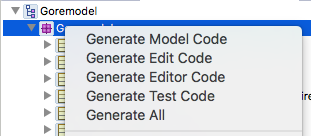
\includegraphics[width=0.5\textwidth]{figuras/unagi/exemplo-gera-codigo.png}
	\caption{Geração automática de código no \eclipse.}
	\label{figura-gera-codigo}
\end{figure}

Rodando na instância do \eclipse a partir do código de editor gerado automaticamente, o plugin \sirius permite que sejam definidos pontos de perspectiva com diferentes especificações de representação gráfica para os objetos do modelo \ecore. Essa especificação é realizada a partir da criação de Projetos de Especificação de Perspectiva (\textit{Viewpoint Specification Project} ou \textit{VSP}), onde são definidos como os elementos serão representados, como suas instâncias serão armazenadas nas classes do metamodelo \ecore, qual o comportamento do modelo quando relações são criadas, dentre outros.

A princípio, é criado dentro do modelo de VSP uma camada (\textit{layer}) que representa a perspectiva a ser representada, nelas são especificados os elementos do modelo \ecore que serão representados, aqui chamados de \textit{Nodes}, que pode ter um estilo padrão ou um estilo condicionado a determinada situação, além disso, pode-se usar formas geométricas predefinidas ou importar imagens externas. 

Como visto na Figura~\ref{exemplo-sirius-vsp}, o elemento \textit{Goal} tem como representação padrão uma elipse amarela. Essa representação pode ser mais bem configurada por meio da paleta de propriedades da mesma (Figura~\ref{figura-propriedades-personalizacao}), onde podem ser especificadas características visuais como cor da linha e tamanho do nome.

\begin{figure}
	\centering
	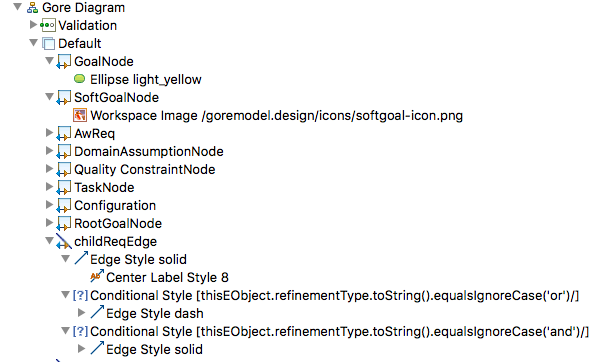
\includegraphics[width=1\textwidth]{figuras/unagi/exemplo-sirius-vsp.png}
	\caption{Sirius Viewpoint Specification Project.}
	\label{exemplo-sirius-vsp}
\end{figure}

\begin{figure}
	\centering
	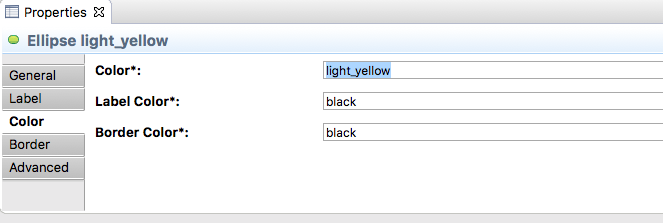
\includegraphics[width=1\textwidth]{figuras/unagi/exemplo-propriedades-personalizacao.png}
	\caption{Propriedades de Representação de Elemento em \sirius.}
	\label{figura-propriedades-personalizacao}
\end{figure}

Na Figura~\ref{exemplo-sirius-vsp} também pode-se observar que além da representação dos \textit{Nodes}, é necessário configurar a criação das linhas de ligação entre os elementos, pois por meio dessas são definidos os refinamentos entre os componentes do modelo. Em \texttt{childReqEdge} é especificado que se um objeto possui tipo de refinamento ``OU'' (``OR''), deve ser usado o tipo de linha tracejada, entretanto, se for do tipo ``E'' (``AND''), usa-se linha contínua. A linguagem usada para escrita de termos condicionais é conhecida como Acceleo Query Language~\cite{musset2006acceleo}, e será posteriormente discuta nesse capítulo.

Além da caracterização dos elementos que serão representados em uma perspectiva, o \sirius também necessita que sejam configuradas propriedades de instanciação dos elementos, assim, além dos \textit{Nodes} de represntação, devem ser criados os \textit{Nodes} de criação, mostrados na Figura~\ref{figura-criacao-node}, onde podem ser observados, por exemplo, a criação do \textit{Node Goal}. Nessa etapa é necessario que primeiramente seja especificado em que tipo de instância do metamodelo o novo objeto será armazenado, para o \textit{Node} de exemplo pode-se observar que há duas ocasiões:
\begin{itemize}
	\item Caso o elemento for o elemento pai, ou seja, a raiz da árvore de representação, deve ser armazenado em uma variável especial da classe \textit{GoalModel}, de nome \textit{rootGoal}. Esse caso é verificado ao checar se a variável ainda não foi definda (\texttt{Case[oclIsUndefined(container.rootGoal)]}).
	\item Caso o elemento for refinamento de qualquer nível do elemento pai, então é guardado na variável \textit{children} da classe \textit{GoalModel}.
\end{itemize}

Decididos os casos, é necessário criar uma instancia da classe relativa ao novo elemento, esse processo é definido por meio das propriedades da opção \textit{Create Instance} (Figura~\ref{figura-criacao-node}). Essas propriedades são definidas de acordo com o modelo \ecore, como pode ser visto na Figura~\ref{figura-propriedades-create-instance}. O campo \textit{referenceName} deve se referir a variável da classe de contenimento que será usada para armazenar o novo elemento, enquanto \textit{Type Name} refere-se à classe do novo componente do modelo.

\begin{figure}
	\centering
	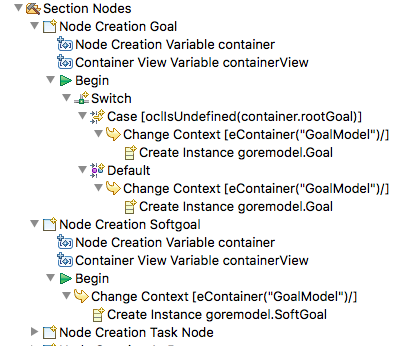
\includegraphics[width=0.7\textwidth]{figuras/unagi/exemplo-criacao-nodes.png}
	\caption{Criação de Nodes no \sirius - Exemplo de criação de nó.}
	\label{figura-criacao-node}
\end{figure}

\begin{figure}
	\centering
	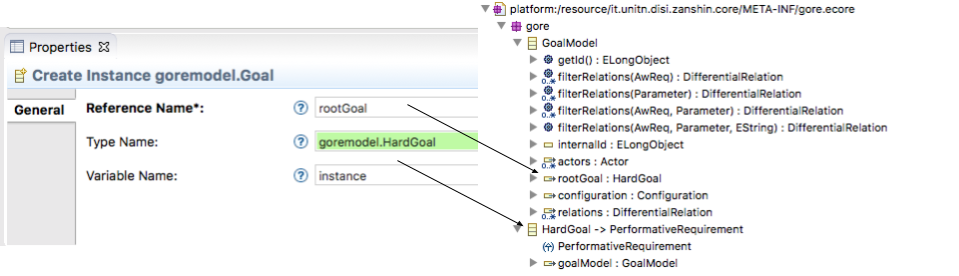
\includegraphics[width=1\textwidth]{figuras/unagi/exemplo-propriedades-create-instance.png}
	\caption{Criação de Nodes no \sirius - Exemplo de criação de instancia de nó.}
	\label{figura-propriedades-create-instance}
\end{figure}

Por fim, foi modelada uma perspectiva diferente para especificação das estratégias de adaptação dos \awreqs, permitindo que cada um tenha sua propria representação em um diagrama separado, com o objetivo de evitar que o modelo principal ficasse ``poluído'' por excesso de informação. 

% ======================================================================================================
% SUBSEÇÃO O Editor Gráfico
% ======================================================================================================
\subsection{O Editor Gráfico}
\label{sec-unagi-apresentacao-editor}

Após todo o processo de detalhamento da representação dos elementos do editor, é possivel então criar um modelo de especificação de perspectiva (\textit{Viewpoint Specification Model}), que permite a criação do diagrama usando recursos de arrastar e soltar, considerados intuitivos por estarem presentes na maioria dos editores gráficos atuais. A Figura~\ref{figura-paleta-unagi} mostra o editor em execução, onde pode ser vista a área de modelagem, bem como a paleta de elementos que podem ser criados, também é mostrada a paleta com tipos de refinamentos disponíveis para modelagem. Esses refinamentos podem ser selecionados e então desenhados apenas clicando no elemento de origem e destino, nesta ordem. As propriedades relativas a cada elemento do modelo podem ser modificadas por meio da paleta de opções que aparece na área inferior do editor (Figura~\ref{unagi-paleta-opcoes}).

\begin{figure}
	\centering
	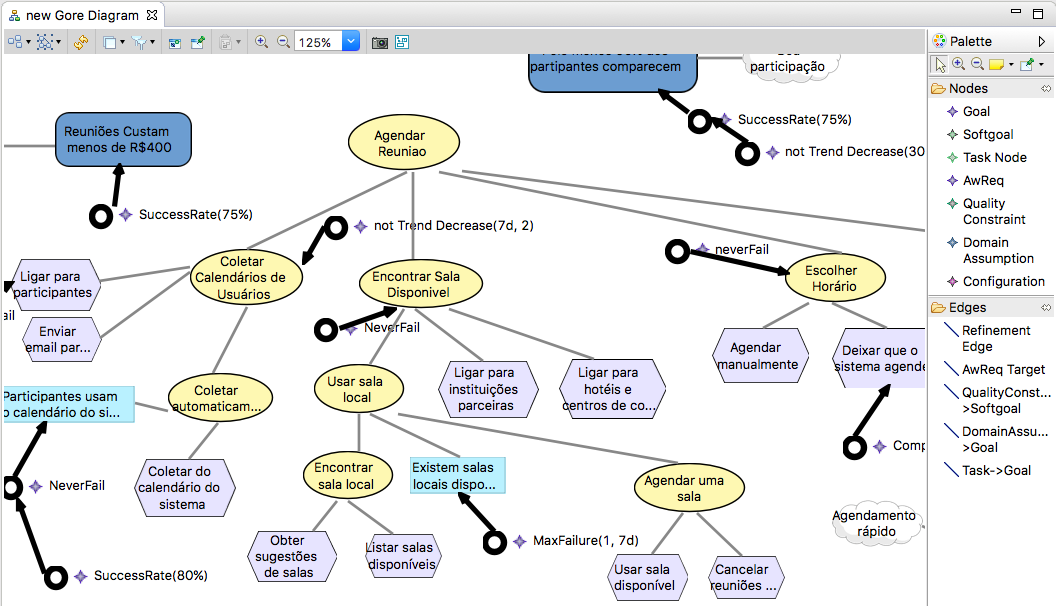
\includegraphics[width=1\textwidth]{figuras/unagi/modeloemunagi.png}
	\caption{Editor Unagi.}
	\label{figura-paleta-unagi}
\end{figure}

\begin{figure}
	\centering
	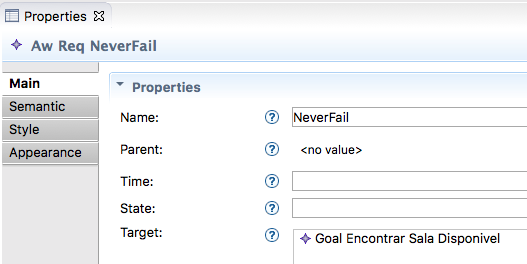
\includegraphics[width=0.85\textwidth]{figuras/unagi/paletaopcoes.png}
	\caption{Editor Unagi - Paleta de Opções.}
	\label{unagi-paleta-opcoes}
\end{figure}

Para acessar a perspectiva que permite o detalhamento dos \evoreqs referentes a cada \awreq é necessário simplesmente um clique duplo sobre o Requisito de Percepção desejado. O editor então oferece a opção de criação de um subdiagrama de detalhamento dos elementos, mostrado na Figura~\ref{figura-subdiagrama-awreq}. Assim, o usuário pode determinar as Condições de Resolução, as Condições de Aplicabilidade e as Estratégias de Adaptação usando a mesma lógica de arrastar e soltar, selecionando os elementos na parte direita da tela. É importante dizer que o modelo só aceita a criação de um elemento específico após seu elemento ``pai'' ter sido criado, por exemplo, só é possível criar uma Estratégia de Adaptação após ter definido uma Condição de Aplicabilidade.

\begin{figure}
	\centering
	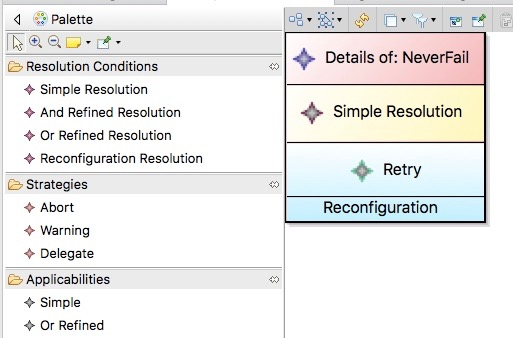
\includegraphics[width=0.85\textwidth]{figuras/unagi/unagisubdiagrama.jpg}
	\caption{Editor Unagi - Subdiagrama de Especificação de \evoreqs.}
	\label{figura-subdiagrama-awreq}
\end{figure}

% ======================================================================================================
% SEÇÃO O Conversor
% ======================================================================================================
\section{Conversor}

\vitor{Faltou esta seção...}

\vitor{Onde pode ser encontrado o código-fonte do Unagi? Antes de você citar a URL do GitHub aqui, acho que deveríamos transferir o repositório para o NEMO. Pode ser?}